\chapter{Background}
\label{ch:Background}

In this chapter, I present the concepts relevant to the subject of the thesis. First, I introduce the topic of MT and the type of architecture I focus on later in the work. Next, I outline the problem of ambiguity and bias in MT models.

% WSD (if I end up using it)
% QE (if I end up using it)

%%%%%%%%%%%%%%%%%%%%%%%%%%%%%%%%%%%%%%%%%%%%%%%%%%%%%%%%%%%%%%%%%%%%%%%%%%%%%%%%%%%%%%%%%%%%
\section{Neural Machine Translation}
\label{sec:Background:NMT}

Machine Translation (MT) is the process of using computer technology to translate text from one natural language to another. This can be achieved using different paradigms. There are three main types of machine translation systems: Rule-based Machine Translation (RBMT), Statistical Machine Translation (SMT) and Neural Machine Translation (NMT). 

Conventional RBMT systems use pre-defined rules based on syntax, morphology and semantics, created by professional linguists. Since language is dynamic and evolves over time, these rules need frequent adaptation, which is costly. However, the key weakness of rule-based translation systems is that they require extensive lexicons and a large set of rules \parencite{SMT_book}. 

SMT systems, on the other hand, use a data-driven approach that utilizes statistical models derived from the analysis of bilingual and monolingual corpora. The quality of SMT output depends heavily on the size and quality of the corpora used to train the models. SMT’s general weakness is that it can only translate a phrase if it exists in the training dataset \parencite{SMT_book}.

Neural Machine Translation (NMT) is a subfield of SMT, which uses an artificial neural network to learn a statistical model for machine translation. Unlike traditional SMT systems, which require a pipeline of specialized components such as language model and translation model, NMT trains its statistical model end-to-end, mapping directly from an input source language to an output target language. NMT can recognize patterns in the training data to determine a context-based interpretation that can predict the likelihood of a sequence of words. Unlike SMT, NMT models are able to learn from each translation task and improve upon each subsequent translation. NMT models are more memory-efficient and also have a higher accuracy than SMT models, which makes them the appropriate choice for creating high-quality MT systems \parencite{NMT_book}.

% TODO: How in deep should I explain the Transformer and NMT?

%%%%%%%%%%%%%%%%%%%%%%%%%%%%%%%%%%%%%%%%%%%%%%%%%
\subsection{Sequence-to-Sequence Modeling}
\label{sec:Background:Seq2Seq}
The task of NMT is typically solved using Sequence-to-Sequence (Seq2Seq) modeling \parencite{seq2seq}. A Seq2Seq model has two parts: an encoder and a decoder. Both work separately and come together to form a large neural network model. This architecture has the ability to handle input and output sequences of variable length. A simplification of the architecture of NMT models can be seen in Fig. \ref{fig:seq2seq}. Firstly, each word in the input sentence is fed separately into the encoder to encode the source sentence into an internal fixed-length representation called the context vector. This context vector contains the meaning of the sentence. Secondly, the decoder decodes the fixed-length context vector and then predicts the output sequence.

\begin{figure}
  \centering
  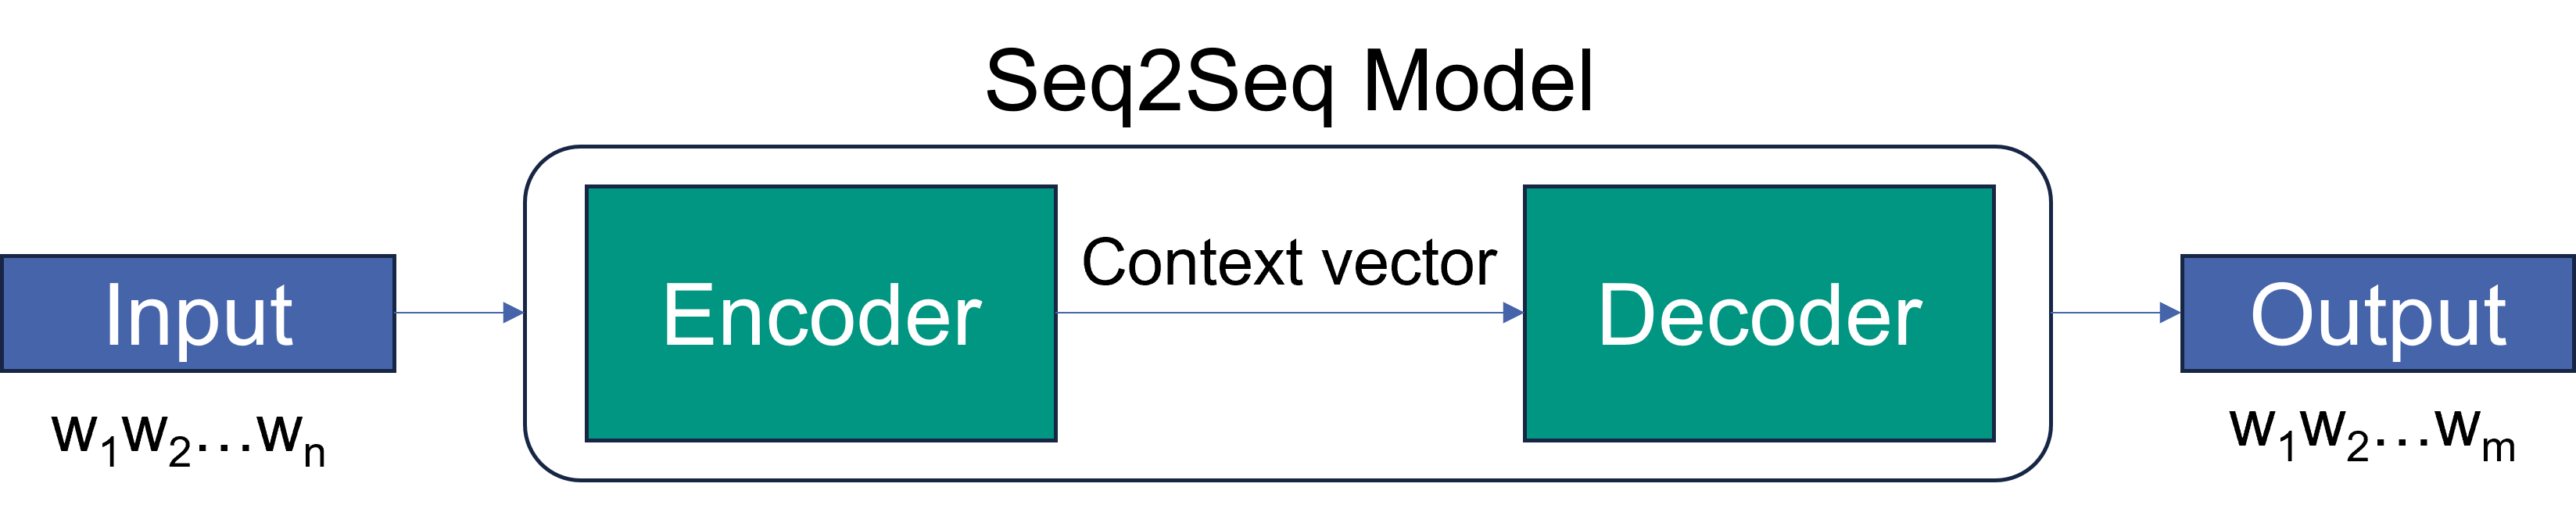
\includegraphics[scale=0.57]{figures/seq2seq.png}
  \caption{Sequence-to-Sequence Modeling}
  \label{fig:seq2seq}
\end{figure}

The original architecture consists of a pair of Recurrent Neural Networks (RNNs) in the roles of encoder and decoder. RNNs process the input sequence token by token, which prohibits parallelization and makes the training and inference slow, especially when processing longer sequences. Also, they suffer from vanishing or exploding gradients, which is inconvenient for effective training. One solution for these problems served Long Short-Term Memory (LSTM) networks, a type of RNN that has additional memory gates to regulate the flow of information through the network better \parencite{lstm}. Despite this, using a fixed-length context vector still incurs a bottleneck in the model. To alleviate this problem, the use of attention-based architectures for neural machine translation was explored \parencite{attention}. 

The attention mechanism allows the decoder to look at the source tokens that are relevant while generating the next token. Despite all these efforts, using RNN-based encoder and decoder still forces the network to handle input sequentially, which makes it difficult to handle long-range dependencies within the input and output sequences from memory. Hence, \cite{transformer} proposed the Transformer architecture, which replaces RNNs with self-attention layers in the Encoder-Decoder network. Since in this work I make use of models based on the Transformer, next I will introduce its basic principle and components.

%%%%%%%%%%%%%%%%%%%%%%%%%%%%%%%%%%%%%%%%%%%%%%%%%
\subsection{Transformer Architecture}
\label{sec:Background:Transformer}
A Transformer is a Seq2Seq model, introduced by \cite{transformer}. An important feature of the Transformer architecture is its attention mechanism. The attention module looks at an input sequence and decides at each step which other parts of the sequence are important, differentially weighting the significance of each part of the input data. Like RNNs, Transformers are designed to handle sequential input data, such as natural language. However, unlike RNNs, Transformers can process the whole input sequence in parallel. The attention mechanism provides context for any position in the input sequence. This feature allows for more parallelization than RNNs and therefore reduces training times significantly \parencite{transformer}.

% Transformer Components
The Transformer architecture as presented in the original paper by \cite{transformer} is depicted in Fig. \ref{fig:transformer}.
The input embedding layer converts the high-dimensional input sequence into a low-dimensional sequence of vectors to capture the meaning and context.
The positional encoding preserves the sequential order of words in the input sentence and can be thought of as the distance of one word to another word in a sequence. This relative position of the words in the sequence is needed since the words are passed in parallel, as opposed to RNNs, which process them in order.
Self-attention is the weighted sum of all other words in the input sequence for each word using similarity (dot product) and SoftMax to focus on the most relevant parts of the input for each element. The multi-head attention repeats self-attention multiple times based on how many encoder/decoder layers there are.

There are multiple encoder and decoder layers. 
Each encoder has one multi-head self-attention, which encodes the weight of the input words to each other. 
Each decoder has one masked multi-head self-attention and one multi-head attention. The masked multi-head self-attention ensures that only words coming before a word are compared to that word, which means it only attends to preceding words in the input sequence during the decoding process. Applying a mask forces the model to ignore future words and focus only on the preceding words during the attention computation. % The mask specifically sets the attention weights to a very large negative value for the positions that correspond to future words, effectively making those weights close to zero after applying the softmax function. 
The multi-head cross-attention module in the decoder compares output tokens to input tokens.
Both the encoder and the decoder have one feed-forward layer, as well as adding and normalizing of residuals at each stage after the attention layers.

The output from the decoder is a vector of length of the input tokens. This output is fed into a fully connected (linear) layer to map it to a set of output prediction and then converted into probability over possible words like multi-class classification using a SoftMax layer.


The Transformer revolutionized NMT by replacing recurrence with attention, which allowed for simultaneous computations and more effective handling of long-range dependencies. This makes them efficient on hardware like GPUs and TPUs and pushes them to be the rational choice for architecture in the realm of MT.

\begin{figure}
  \centering
  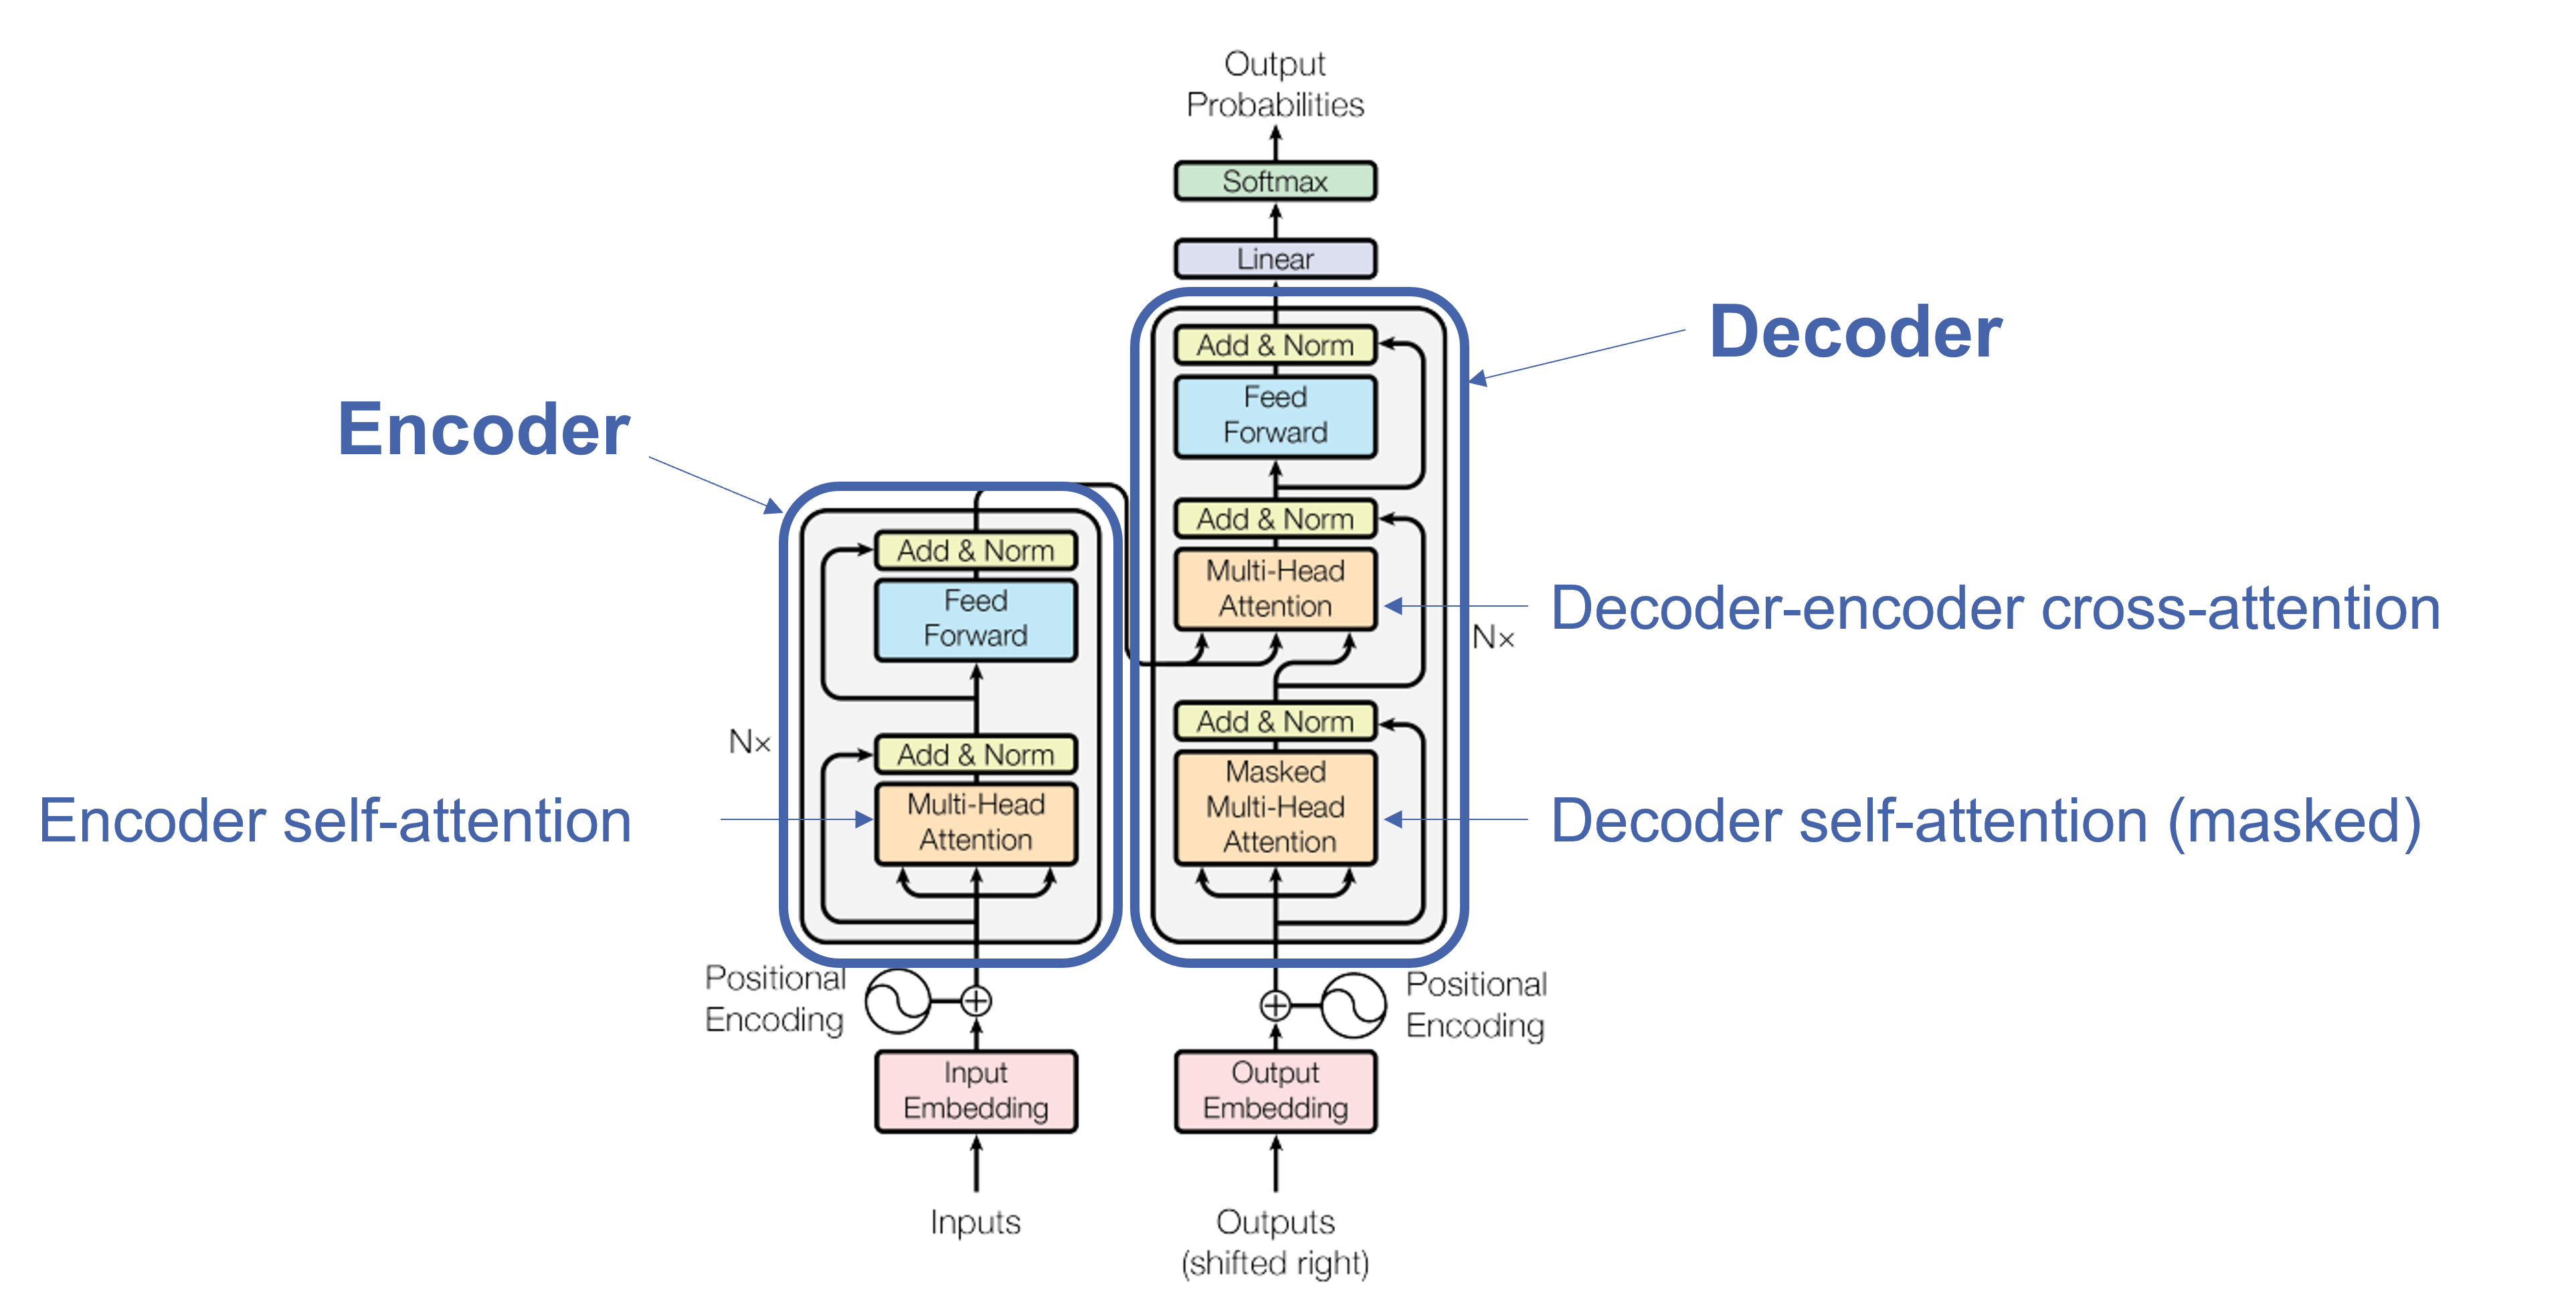
\includegraphics[scale=0.5]{figures/transformer.png}
  \caption{The Transformer Architecture}
  \label{fig:transformer}
\end{figure}

% Explain autoregressive sampling?

%%%%%%%%%%%%%%%%%%%%%%%%%%%%%%%%%%%%%%%%%%%%%%%%%%%%%%%%%%%%%%%%%%%%%%%%%%%%%%%%%%%%%%%%%%%%
\section{Ambiguity and Bias in Machine Translation}
\label{sec:Background:Ambiguity_Bias}
Biases present in AI systems are an important problem stemming from cultural and historical issues present in the data from which models are learning. The developed systems in turn reinforce the present societal prejudices and old social norms, instead of mitigating them. 
It is important to understand how these biases occur in translation and to differentiate the different types of bias one may face.

Next, I will define the concepts of ambiguity and bias.

\paragraph{Ambiguity}
Ambiguity refers to the quality of being open to more than one interpretation, as in not having one obvious meaning. It is the type of meaning in which a phrase, statement, or resolution is not explicitly defined, making several interpretations plausible. A common aspect of ambiguity is uncertainty. In MT, ambiguity occurs when the source text leaves some essential properties unspecified, but the target language requires the property to be specified for correct translation. 

The ambiguity can be \textbf{resolvable} or \textbf{unresolvable}. It is resolvable when some semantic property required for the subject to be disambiguated can be found in the context, which defines the rest of the text available to the translation system. On the other hand, it is unresolvable, when no property necessary for disambiguation can be inferred from the context. To illustrate these two cases, we will look at two examples. When translating the sentence "She is a doctor." from English to German, which has no gender-neutral word for "doctor", the translation system has to choose the male ("Arzt") or female ("Ärztin") gender word for "doctor". In this case, the word "doctor" is ambiguous. However, the gender is resolvable from context due to the presence of the female pronoun "she". In contrast, the example sentence "I am a doctor." also contains the ambiguous word "doctor", but it is not indicated in the rest of the text whether the intended referent of "I" and "doctor" is a man or a woman. This makes the ambiguity in this case unresolvable \parencite{bias_taxonomy}.

When the ambiguity is unresolvable, the translation system cannot make an informed decision and instead applies randomness or previously acquired knowledge in choosing the translation, making an \textbf{unjustified assumption}. The assumption is unjustified because nothing actually present in the source text justifies it. In the example of "I am a doctor." the translator typically decides for the male translation of the word "doctor", because this case appears most often in similar contexts in its training data. Although, context allows for two possible translations in German for the ambiguous word "doctor", the system will consistently prefer the male translation, which leads to a \textbf{bias}. 

\paragraph{Bias}
Bias refers to a disproportionate weight in favor of or against an idea or thing, usually in a way that is closed-minded, prejudicial, or unfair. In machine translation, it is the tendency to make certain unjustified assumptions more often than others. Biases stem from unresolved ambiguities leading to unjustified assumptions and can be categorized as follows \parencite{bias_taxonomy}:
\begin{itemize}
    \item \textbf{Gender bias}: This type of bias occurs when there is an unresolvable ambiguity relating to the gender of people. Some commonly gender ambiguous words are professions such as doctor, teacher, cleaner. 
    \item \textbf{Number bias}: This bias presents itself when the English pronoun "you" has an unresolvable ambiguity concerning whether it refers to a single person ("du" in German) or multiple people ("ihr" in German). 
    \item \textbf{Formality bias}: This bias occurs when the English pronoun "you" has an unresolvable ambiguity concerning whether the subject is addressed formally ("Sie" in German) or informally ("du" in German). 
\end{itemize}

A MT system is biased if, while dealing with unresolvable ambiguities and deciding which unjustified assumptions to make, its decisions are not random. This means that the system makes certain unjustified assumptions more often than others. For example, if it consistently translates the occupation "doctor" as male, then the translator is biased \parencite{bias_taxonomy}.


% TODO: Types of languages

\parencite{Savoldi_2021}


% Available literature focuses on gender bias

%%%%%%%%%%%%%%%%%%%%%%%%%%%%%%%%%%%%%%%%%%%%%%%%%
\subsection{Bias Detection in Machine Translation}
\label{sec:Background:Bias_Detection}

% For bias detection we need:
% - Challenge sets are artificially created usually small datasets that represent some gender-related issue, such as assigning the right pronoun to a specific role
% - Automatic evaluation methods needed, because the BLEU score, normally used for assessing the quality of translations, cannot judge on the occurrence of bias [Stanovsky2019]


%%%%%%%%%%%%%%%%%%%%%%%%%%%%%%%%%%%%%%%%%%%%%%%%%
\subsection{Bias Mitigation in Machine Translation}
\label{sec:Background:Bias_Mitigation}

% Bias mitigation methods: data modification, word embeddings, architecture modification
% - Modification of the data [Costa2019]
% - Debiasing word embeddins [Zhao2018] [Bolukbasi2016]
% - Model debiasing through metadata about gender [Vanmassenhove2018]



Man is to computer programmer as woman is to
homemaker? debiasing word embeddings \parencite{bolukbasi2016man}
- Hard-debiased embeddings: post-process method for debiasing word embeddings
- Downsides: pipeline approach propagates errors; completely removes gender information from words; 
- Downsides: pipeline approach propagates errors; completely removes gender information from words;  remove valuable information in the embeddings for semantic relations between words with several meanings that are not related to the bias being treated

Men Also Like Shopping: Reducing Gender Bias Amplification using Corpus-level Constraints \parencite{Zhao_2017}
- WinoBias dataset: composed of pro-stereotype (PRO) and anti-stereotype (ANTI) subsets

Gender bias in coreference resolution: Evaluation and debiasing
methods \parencite{Zhao_2018_coreference}

Assessing gender bias in machine translation: a case study with Google Translate \parencite{Prates_2019}
- list of occupations

Getting Gender Right in Neural Machine Translation \parencite{Vanmassenhove_2018}
- develop gender-informed MT models; model debiasing through metadata
- compile a large multilingual dataset on the politics domain that contains the speaker information
- incorporating it into a MT system improves the translation quality

Neural Machine Translation Doesn't Translate Gender Coreference Right Unless You Make It \parencite{Saunders_2020_coreference}
- explore the use of word-level gender tags

Reducing Gender Bias in Neural Machine Translation as a Domain Adaptation Problem \parencite{Saunders_2020}
- propose to post-process the MT output with a lattice re-scoring module
- counterfactual data augmentation
 
Decoding and diversity in machine translation \parencite{roberts2020decoding}

GeBioToolkit: Automatic extraction of gender-balanced multilingual corpus of Wikipedia biographies \parencite{costa2019gebiotoolkit}
- fine-tuning on gender-balanced datasets based on Wikipedia biographies
- Downside: does not mitigate stereotyping harms, as it does not account for the qualitative different ways in which men and women are portrayed

On Measuring Gender Bias in Translation of Gender-neutral Pronouns \parencite{Cho_2019}

Automatically identifying gender issues in machine translation using perturbations \parencite{Gonen_2020}

"You sound just like your father": Commercial machine translation systems include stylistic biases \parencite{Hovy_2020}
- conjecture the existence of age and gender stylistic bias due to models’ under-exposure to the writings of women and younger segments of the population

Gender in danger? evaluating speech translation technology on the MuST-SHE corpus \parencite{MuST-SHE}

Fine-tuning Neural Machine Translation on Gender-Balanced Datasets \parencite{costa2020fine}


!Learning Gender-Neutral Word Embeddings \parencite{Zhao_2018_GN-GloVe}
- propose a training procedure for learning gender-neutral word embeddings
- Gender-Neutral variant of GloVe (GN-GloVe): training word embedding models with protected attributes (e.g., gender)

!Equalizing Gender Bias in Neural Machine Translation
with Word Embeddings Techniques \parencite{Escud_Font_2019}
- study the presence of gender bias in MT and give insight on
the impact of debiasing in such systems
- proposed a gender-debiased approach for NMT
- specific analysis based on correference and stereotypes to evaluate the effectiveness of our technique
- evaluate proposed system on the WMT English-Spanish benchmark task
- bilingual English-Spanish Occupations test set
- verified hypothesis that consisted on the fact that if the translation system is gender biased, the context is disregarded, while if the system is neutral, the translation is correct (since it has the information of gender in the sentence).

!Evaluating Gender Bias in Machine Translation \parencite{Stanovsky_2019}
- present the first challenge set (WinoMT) and evaluation protocol for the analysis of gender bias in machine translation (MT)
- devise an automatic gender bias evaluation method for eight target languages with grammatical gender, based on morphological analysis
- evaluate  four popular industrial MT systems and two recent state-of-the-art academic MT models (Google Translate, Microsoft Translator)
- use data introduced by two recent coreference gender-bias studies: the
Winogender \parencite{Rudinger_2018_coreference}, and the WinoBias \cite{Zhao_2018_coreference} datasets
- WinoMT: concatenating Winogender and WinoBias; equally balanced between male and female genders as well as between stereotypical and non-stereotypical gender-role assignments (e.g., a female doctor versus a female nurse)
- Measures: gender accuracy, difference in performance between male and female, difference in performance between stereotypical and non-stereotypical gender role assignments
- Fighting bias with bias: automatically creating a version of WinoMT with the adjectives “handsome” and “pretty” prepended to male and female entities, respectively -> not applicable in a real-world scenario
- Downsides: synthetic samples - controlled experiment environment, but may introduce some artificial biases; only English as source language; too small set for training easy to overfit

!Literature review: Gender Bias in Machine Translation \parencite{Savoldi_2021}
- critically review current conceptualizations of bias in light of theoretical insights from related disciplines
- summarize previous analyses aimed at assessing gender bias in MT
- discuss the mitigating strategies proposed so far
- point toward potential directions for future work


%%%%%%%%%%%%%%%%%%%%%%%%%%%%%%%%%%%%%%%%%%%%%%%%%%%%%%%%%%%%%%%%%%%%%%%%%%%%%%%%%%%%%%%%%%%%
% In Progress:
% - Unsupervised Word Sense Disambiguation (WSD) may help discover biased words
% WSD: technique in natural language processing (NLP), defined as the ability to determine which meaning of word is activated by the use of word in a particular context
% - Researching methods for Quality Estimation (QE) for detecting biases in translation
% QE: method for predicting the quality of a given translation rather than assessing how similar it is to a reference segment, E.g. multiple beams in Beam search: low confidence = high confidence for error in translation